\chapter{Templates}

\begin{figure}[htb]
\centering
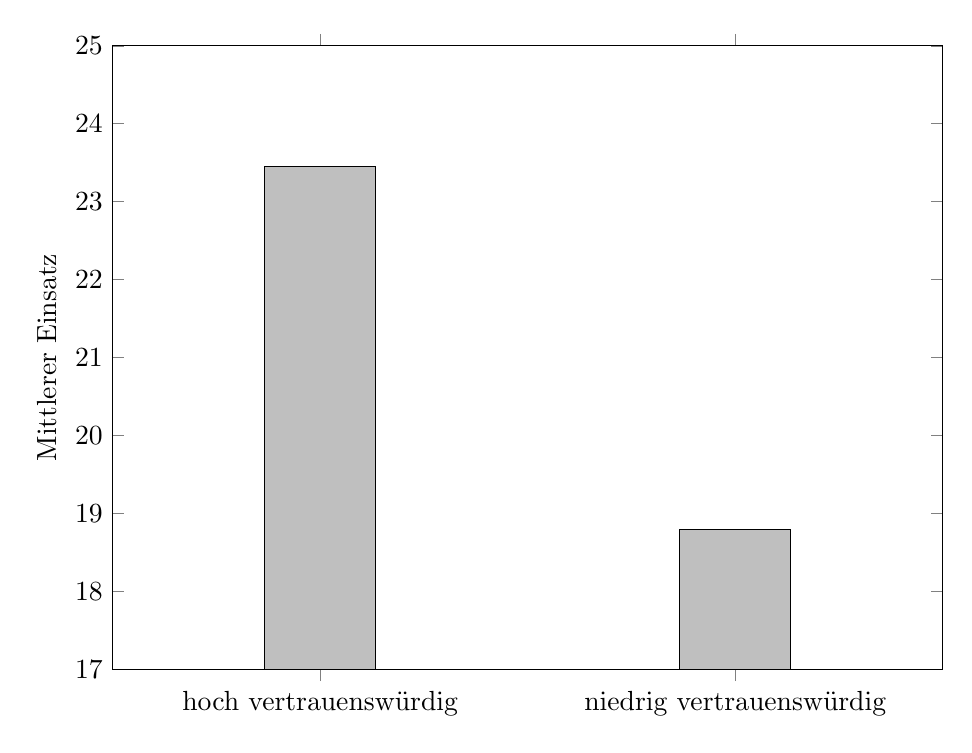
\begin{tikzpicture}
  \begin{axis}[
    width=\textwidth,
    height=9.5cm,
    ybar=0pt, % Raum zwischen den Balken
    bar width=40pt,
    enlarge x limits=0.5,
    legend style={at={(1,1.15)},anchor=north east,draw=none},% Legende über Abb.
    legend cell align=left,% Linksbündige Ausrichtung der Legende
    % xlabel={Gesicht},
    xtick={data},
    symbolic x coords={hoch vertrauenswürdig,niedrig vertrauenswürdig},
    ymin=17,
    ymax=25,
    ylabel={Mittlerer Einsatz},
    %ytick={17,18,...,25}
  ]
    \addplot[
        black,fill=lightgray
      ]coordinates {
      (hoch vertrauenswürdig,23.453) 
      (niedrig vertrauenswürdig,18.797)
    };
    % \addlegendentry{~betrügerisches Verhalten};
    % \addplot[
    %     black,fill=white,
    %     postaction={pattern=north east lines,pattern color=gray}
    %     ] coordinates {
    %   (hoch vertrauenswürdig,22.891) +- (0,0.410)
    %   (niedrig vertrauenswürdig,18.844) +- (0,0.407)
    % };
    % \addlegendentry{~kooperatives Verhalten};
  \end{axis}
\end{tikzpicture}
\caption{Investitionsverhalten. Die Fehlerbalken stellen die Standardfehler dar.}
\label{fig:Investitionsverhalten}
\end{figure}

\begin{figure}[H]
	\centering 
	\includegraphics[width=\textwidth]{img/Production_IST.png}	\caption[TEST]{\label{fig:logo}test
	}
\end{figure}


\begin{figure}[H]
	\centering 
	\includegraphics[width=\textwidth]{img/Arch_IST.png}	\caption[TEST]{\label{fig:logo}test
	}
\end{figure}

\begin{figure}[H]
	\centering 
	\includegraphics[angle=270,width=\textwidth]{img/Arch_SOLL.png}	\caption[TEST]{\label{fig:logo}test
	}
\end{figure}

\begin{figure}[H]
	\centering 
	\includegraphics[angle=270,width=\textwidth]{img/Order_Operating_IST.png}	\caption[TEST]{\label{fig:logo}test
	}
\end{figure}

\begin{figure}[H]
	\centering 
	\includegraphics[angle=270,width=\textwidth]{img/Order_Operating_SOLL.png}	\caption[TEST]{\label{fig:logo}test
	}
\end{figure}

\begin{figure}[H]
\centering 
\lstinputlisting[style=JavaScriptStyle, caption=test.js]{code/test.js}
\end{figure}

\begin{figure}[H]
\centering 
\lstinputlisting[style=JavaStyle, caption=test.java]{code/test.java}
\end{figure}

\begin{definitionForm}[Definition]
Diese Hervorhebungen können für deine Arbeit an machen stellen sehr nützlich sein. Besonders bei Definitionen macht es einen guten Eindruck, wenn diese in solch einer Form dargestellt ist. 
\end{definitionForm}

DHBW Richtlinie: Laut den aktuellen Angaben der DHBW sind diese Boxen nicht notwendig. Helfen können sie jedoch, um einen Faktor speziell hervorzuheben. Bitte beachte, dass deine Projektarbeit oder auch Bachelorarbeit kein Bilderbuch ist! Alles was eingebunden wird sollte schlicht und dezent dargestellt sein.

\begin{attentionForm}[Wichtig] Verwende kein \glqq ich\grqq{}, während der gesamten Arbeit. Jeder weiß, dass es deine Arbeit ist. Auch von Sätzen mit \glqq man\grqq{}, solltest du Abstand nehmen. Frage deinen Betreuer gerne, welche Vorzüge er oder sie hat. Jeder Dezi oder DHBW-Betreuer hat in diesem Zusammenhang unterschiedliche Meinungen.
\end{attentionForm}

\autocite{Staud2006Geschaftsprozessanalyse:Standardsoftware}



\begin{table}[H]
	\centering
	\begin{tabularx}{\textwidth}{|l|X|} 
		\hline
		Auslöser                                     &   
		Der Produktionsplaner möchte Engpässe an betroffenen Arbeitsplätzen durch Modifikationen an Kapazitätsangeboten beheben. \\ 
		\hline\hline
		Input                                         &   
		Handlungsbedarf durch die Auswertung der Kapazitätsauslastung \\ 
		\hline\hline
		Aktivitäten &   
		\begin{minipage}{5in}
    		\begin{enumerate} 
        		\renewcommand{\labelenumi}{(\arabic{enumi})}
        		\item Starten der Anwendung
        		\item Iterative Vorgehensweise bis zur Zielerreichung:
            		\begin{enumerate} 
            		\renewcommand{\labelenumi}{(\arabic{enumi})}
            		\item Wahl einer Arbeitsplatzkapazität
            		\item Erstellung einer Angebotskapazität
            		\item Festlegung eines Gültigkeitszeitraums
            		\item Pflege von Schichten in der Angebotskapazität
            		\item Speichern der Änderungen
            		\end{enumerate}
            	\item Ende des Prozesses
    		\end{enumerate}
    		\vspace{1pt}		
		\end{minipage} \\
		\hline\hline
		Output                                        &   
		Modifizierte Kapazitätsangebote von Arbeitsplätzen  \\
		\hline
	\end{tabularx}
	\caption{\label{tab:aktivitäten}Ist-Prozessbeschreibung }
\end{table}

\begin{table}[H]
	\centering
	\begin{tabularx}{\textwidth}{l X} 
		\toprule
		\textbf{Kriterium}  &   
		\textbf{Beschreibung}  \\ 
		\midrule
		VP1 &   
		Keine Modifikationsmöglichkeiten  \\  \cmidrule(r){1-1} \cmidrule(r){2-2}
		VP2 &   
		Unausgereifter Prozessablauf \\ \cmidrule(r){1-1} \cmidrule(r){2-2}
		VP3 &   
		Mangelhafte Bedienbarkeit  \\ \cmidrule(r){1-1} \cmidrule(r){2-2}
		VP4 &   
		Kontraintuitives Stammdatenmodell  \\ \cmidrule(r){1-1} \cmidrule(r){2-2}
		VP5 &   
		Keine Überprüfung der Validität der Eingaben  \\ \cmidrule(r){1-1} \cmidrule(r){2-2}
		VP6 &   
		Kein Überblick über getätigte Modifikationen  \\
	    \bottomrule
	\end{tabularx}
	\caption{\label{tab:potentiale}Verbesserungspotentiale des Ist-Systems}
\end{table}
